\chapter{Marco teórico}
Con el desarrollo del sistema producto del presente trabajo terminal se involucran ciertos conceptos provenientes en su mayoría de ramas de ciencias de la computación y en general en alusión a la Inteligencia Artificial, por lo que es conveniente dar contexto sobre los elementos necesarios para el desarrollo del trabajo terminal.
\section{Análisis de Imágenes}\label{imAnalysis}
        El análisis de imágenes comprende un conjunto de operaciones sobre una o varias imágenes con el propósito de obtener una imagen con mayor realce o para extraer características útiles, es un tipo de dispensación de señales en el que la entrada es una imagen y la salida puede ser otra imagen o características asociadas a la imagen, algunos de los pasos generales se describen a continuación:
        
        \subsection{Preprocesamiento}
            Preprocesamiento es un nombre común para operaciones con imágenes al más bajo nivel de abstracción. Tanto entrada como salida son imágenes de intensidad. Estas imágenes tienen el mismo tipo de datos que la original, con una imagen de intensidad usualmente representada por una matriz de valores de función de imagen (Brillo) El objetivo de preprocesar es la mejora de los datos de la imagen que borre distorciones o realce características importantes para procesamiento posterior, incluso las transformaciones geométricas de las imagenes e.g (rotación, escalamiento y traslación) son también clasificadas como métodos de preprocesamiento, ya que técnicas similares son utilizadas \cite{imgAnalySeg}.
               
                
        \subsection{Realce de la imagen}
            El objetivo principal de realce de imagen es también procesar una imagen dada tal que el resultado sea mas ajustable que la imagen original para aplicaciones específicas. Por ejemplo para la remoción de ruido.
            \\\\%\bigskip
            Acentúa o afina características de la imagen como ejes, límites o contraste para hacer un despliegue gráfico mas útil para el análisis.
            \\\\%%\bigskip
            El realce no incrementa o decrementa el contenido de la información inherente de los datos pero sí incrementa el rango dinámico de las características elegidas de tal modo que puedan ser detectadas fácilmente.
            \\\\%\bigskip
            Proveé \'mejor\' entrada para otras técnicas avanzadas de procesamiento automatizadas de imágenes.
                        
        \subsection{Segmentación de la imagen}
            El término segmentación utilizada en el contexto de análisis de imágenes se refiere a la partición de una imagen en un conjunto de regiones que la cubren. El objetivo en muchas de las tareas es que para las regiones se representen áreas significativas de la imagen, como áreas urbanas, fronteras o bosques de una imagen satelital. En otras tareas de análisis, las regiones pueden ser conjuntos de bordes de pixeles agrupados en estructuras como segmentos de líneas y segmentos de arcos circulares en imágenes de objetos industriales en 3D. Las regiones pueden también estar definidas como grupos de pixeles teniendo ambos un borde y una forma particular como un circulo o una elipse or polígono. Cuando las regiones de interés no cubren la imagen completa, aún se requiere el proceso de segmentación en regiones de y de fondo para ignorarse. 
            \cite{imgAnalySeg}
            %REF courses.cs.washington.edu/courses/cse576/book/ch10.pdf
            \begin{figure}[H]
                \centering
                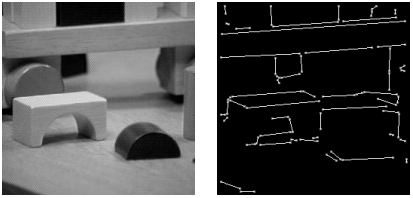
\includegraphics[width=0.7\textwidth]{capitulo2/images/segmentation.PNG}
                \caption{Imagen con bloques (Izquierda) y conjunto de segmentos de linea extraídos (Derecha).}
                \label{fig:segmentacion}
            \end{figure}
        %\subsection{Extracción de características}
            
            %http://citeseerx.ist.psu.edu/viewdoc/download?doi=10.1.1.375.6848&rep=rep1&type=pdf
        %\subsection{Clasificación e interpretación}
            %http://citeseerx.ist.psu.edu/viewdoc/download?doi=10.1.1.375.6848&rep=rep1&type=pdf


\newpage
\section{Deep Learning}
	
El aprendizaje profundo o \textit{deep learning} es una rama del aprendizaje automático (\textit{machine learning} en inglés) que intenta modelar abstracciones de alto nivel a través de complejas arquitecturas computacionales que admiten transformaciones no lineales. El deep learning es la evolución de las ya conocidas redes neuronales las cuales experimentaban problemas de desvanecimiento del gradiente si se usaban demasiadas capas. Con las nuevas técnicas propuestas en el deep learning se logro evitar este problema y así, poder entrenar arquitecturas de millones de parámetros. \\

El perceptrón multicapa (MLP) es el modelo más básico y aún así uno de los más útiles en el campo de las redes neuronales. Su principal objetivo es tratar de aproximar una función $f^{*}$. En el caso del \textit{aprendizaje supervisado}, la función $f^{*}$ toma la forma $y^{*} = f^{*}(x)$ de donde x es un parámetro de entrada que puede ser desde un simple número hasta un tensor y $y^{*}$ es la salida de la función. Entonces, una red neuronal que quiera aproximar $f^{*}$ definirá una función de mapeo de la forma $y = f(x,\theta)$ y aprenderá los parámetros $\theta$ (usualmente conocidos como $W$ y $b$) que dan como resultado la mejor aproximación de tal forma que $y \approx y^{*}$. \\

Las redes neuronales profundas son llamadas redes porque pueden representarse mediante la composición de varias funciones de mapeo. Es decir, un MLP que quiera aproximar una función puede expresarse como $y^{n} = f^{n}(y^{n-1}, \theta^{n})$ con $y^{1} = f^{1}(x, \theta^{1})$ y $n$ siendo la profundidad de la red. 

	\subsection{Gráfos computacionales}
	Para describir con formalidad a las redes neuronales es preciso utilizar una notación que pueda ser expresada a través de gráfos. Según \cite{deeplearningbook} se puede indicar cada nodo del gráfo como una variable que puede ser un tensor para no perder generalidad. 
	
	Para terminar con la definición de estos gráfos, es necesario introducir el concepto de operación, la cual simplemente es una función entre dos o mas nodos del gráfo. Sin perder generalidad, se dice que una operación retorna únicamente una variable, es decir, un solo nodo.
	
	En la Figura \ref{fig:grafo-computacional} se puede ver un ejemplo de un perceptrón de una sola capa que es representado mediante un gráfo computacional. Gracias a esta definición, se puede extender facilmente el gráfo mostrado en \ref{fig:grafo-computacional} para modelar a un perceptrón de $n$ capas.
	
	\begin{figure}[h]
		\centering
		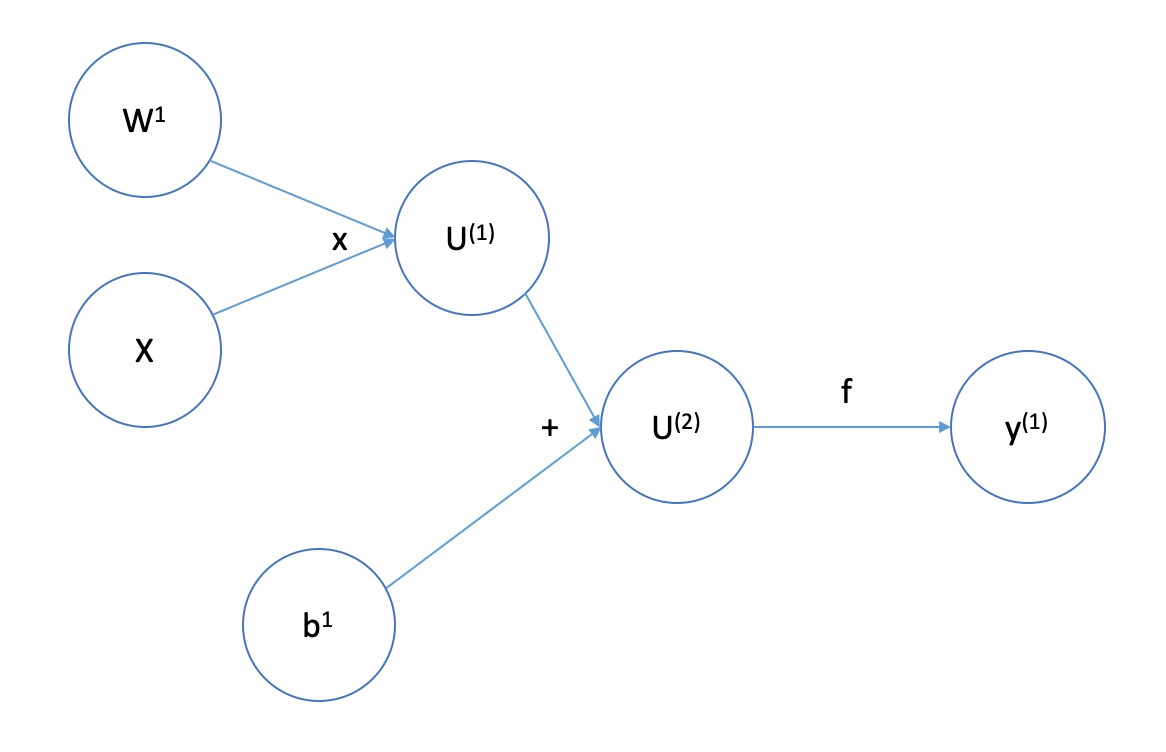
\includegraphics[width=10cm]{capitulo2/images/grafo}
		\caption{Ejemplo de un perceptrón de una sola capa representado mediante un gráfo computacional, siendo $x$ la entrada, $w^{1}$ la matriz de pesos, $b^{1}$ la matriz de bias, $u^{(1)}$ y $u^{(2)}$ nodos intermedios en el gráfo y $y^{1}$ la salida de la red.}
		\label{fig:grafo-computacional}
	\end{figure}

	%\subsection{Algoritmos de aprendizaje}
    
    \subsection{Redes Neuronales Convolucionales}
    
    Las redes neuronales convolucionales también llamadas convolutivas (CNN), son una arquitectura especial de redes neuronales que permite el procesamiento de datos que tengan una estructura de grilla. Algunos ejemplos de esta estructura son: una serie de tiempo es una grilla 1D o una imágene, la cual puede ser vista como una grilla 2D de pixeles. Se puede decir, que una red convolutiva no es más que una red neuronal que utiliza la operación de convolución en lugar de una multiplicación tensorial normal \cite{deeplearningbook}. \\
    
    La operación de convolución que se utiliza en matemáticas e ingeniería esta definida de la siguiente manera:
    
    \begin{equation}
    	y(t) = \int_{-\infty}^{\infty} x(\tau)w(t-\tau)d\tau
    \end{equation}
    
    En terminolgía de las CNN $x$ es la entrada a la red, $w$ es llamado el \textbf{kernel} o \textbf{filtro} y $y$ el mapa de características. \\
    
    Propiamente en los sitemas computacionales no se pueden tener funciones continuas, estas tienen que ser discretas, por lo tanto la operación de convolución que una CNN utiliza es:
    
    \begin{equation}
    	y(t) = \sum_{\tau = -\infty}^{\infty} x(\tau)w(t-\tau)
    \end{equation}
    
    Naturalmente, si lo que se esta trabajando es una imagen, tenemos que aplicar la operación de convolución en dos ejes, es decir:
    
    \begin{equation}
    	y(i,j) = \sum_{m}\sum_{n} x(i,j)w(i-m, j-n)
    \end{equation}
    
    En la Figura \ref{fig:CNNFilter} se puede ver un ejemplo de cómo una imagen es procesada por la etapa de convolución en una CNN.
    
    \begin{figure}[H]
    	\centering
    	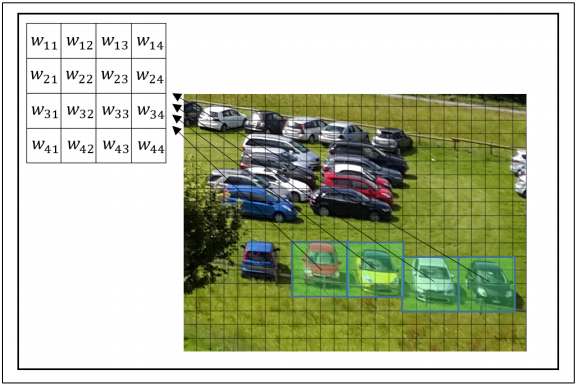
\includegraphics[width=0.7\textwidth]{capitulo2/images/CNN_window.png}
    	\caption{Matriz de pesos conocida como kernel o filtro aplicada a una imagen.}
    	\label{fig:CNNFilter}
    \end{figure}
    
    \subsubsection{Pooling}
    Es una de las operaciones adicionales que se implementan en las CNN. En general se puede establecer que una típica capa convolucional tiene tres partes:
    
    \begin{enumerate}
    	\item Operación de convolución: Es donde utiliza una entrada y la convoluciona con un filtro $w$.
    	\item Función de activación: A veces es llamada fase de detección. Consiste en aplicar una función $f$ al resultado de la primera etapa para modificar la salida y volverla no lineal.
    	\item Etapa de Pooling: Es una manera de modificar aún más la salida de modo que se incremente la significancia estadística de los datos extraidos.
    \end{enumerate}

	La operación de pooling permite que la red sea tolerante a traslaciones y rotaciones leves de la imagen. Por ejemplo, se puede aplicar la función \textit{max pooling} a cada uno de los valores de $f(W*h)$ para obtener una generalización de los datos más importantes observados por la etapa de detección. \\
	
	Una manera efectiva de reducir el tamaño de los datos que la red tiene que procesar a través de sus capas, es utilizar la operación pooling para remuestrear. Esto se logra definiendo una ventana a la que la que se le aplicará la operación. Esta técnica también permite que algunas CNN puedan procesar imágenes de longitud variable.
    
    \newpage
    
   	
\section{Redes Neuronales Recurrentes}

Las redes neuronales recurrentes (RNNs) son una familia de redes neuronales especializadas en procesar secuencias de datos. Es decir, pueden procesar entradas de la forma: $x^{(1)}, x^{(2)}, \dots, x^{(t)}$. Esta particular arquietectura, permite modelar secuencias de datos de longitud variable que serían imprácticas para cualquier otra arquitectura. \\

Las RNNs modelan sistemas dinámicos, es decir, que cada instante $t$ tenemos un sistema $s(t)$ con un estado diferente. Para que los siguientes estados del sistema tengan información de los estados pasados, las RNNs tienen al menos una conexión que es recurrente, es decir, que depende de un estado anterior o en algunos casos de estados futuros. \\

Una de sus principales ventajas es la compartición de parámetros. Esto quiere decir que para diferentes estados del sistema, podemos aplicar los mismos parámetros $\theta$, permitiendo así, entrenar solo un conjunto de parámetros para todo el sistema en vez de un conjunto particular para cada estado. \\

En la Figura \ref{fig:rnn} se puede apreciar un ejemplo de una RNN que cuya ecuación es: $s(t) = f(s^{(t-1)}, \theta)$. Como se han definido las redes neuronales en términos de gráfos, es posible utilizar el algoritmo de back-propagation para calcular los gradientes de cada estado. Normalmente cuando se aplica back-propagation a una RNN se le conoce como back-propagation through time (BPTT). \\

\begin{figure}[H]
	\centering
	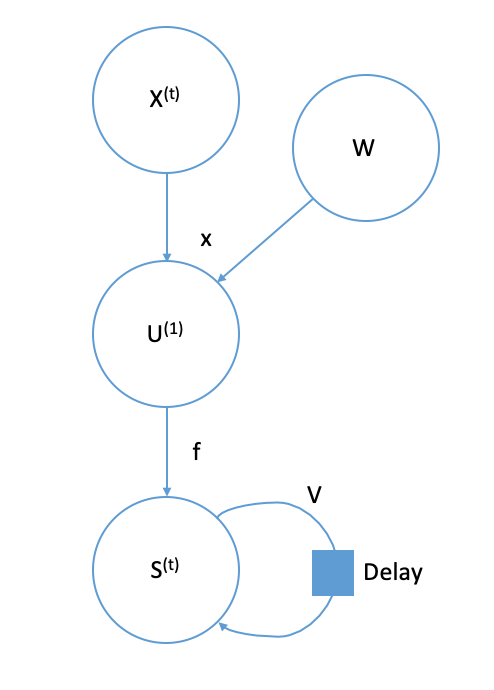
\includegraphics[width=4cm, height=5.5cm]{capitulo2/images/rnn}
	\caption{Ejemplo de una RNN que modela la ecuación $s(t) = f(s^{(t-1)}, \theta)$, donde $\theta$ representa los parámetros $W$ y $V$, $f$ la función no lineal aplicada a $Wx^{(t)}$ y $V$ la matriz de pesos aplicada a $s^{(t-1)}$.}
	\label{fig:rnn}
\end{figure}

La manera que tiene una RNN para poder procesar una secuencia de longitud variable y brindar información respecto de ella, es a través de los estados $s(t)$ ya que estos si tienen una longitud fija. De este modo se puede decir que funcionan muy parecido a una CNN, ya que sumarizan las características de la secuencia hasta el momento $t$. Para realizar alguna predicción final, normalmente se utiliza algúna otra capa que efectue una función $f$, justo como lo hacen las CNNs. \\
  
    \subsection{Arquitectura Encoder-Decoder}
    Esta arquitectura de RNN se ha vuelto muy popular pues permite a una red procesar secuencias de longitud variable y obtener como resultado secuencias de longitud variable. Este tipo de problemas son conocidos como problemas sequence-to-sequence. Algunos ejemplos de problemas de este estilo son el reconocimiento del habla en tiempo real o el reconocimiento de la escritura. \\
    
    La arquitectura se compone de dos redes recurrentes, la primera es denominada el \textit{encoder}, el cual es una red que 'codifica' la entrada $x^{(t)}$. Si lo que se quiere es codificar una serie de tiempo, normalmente se usará una RNN y como salida será la señal $s(t)$. En este tipo de redes a la señal $s(t)$ se le conoce como el contexto $C$. \\
    
    La segunda red que compone a la arquitectura es el \textit{decoder}, el cual toma como entrada el contexto $C$ generado previamente por el encoder y lo utiliza para generar la secuencia de salida. El decoder es en general una RNN.
    
    \subsection{Long Short-Term Memory}
   	Hasta ahora, las arquitecturas más exitosas para procesar secuencias son las llamadas Gated RNN. Estas redes permiten aprender secuencias muy largas o que requieran memorizar mucha información. El problema que existía, era que el gradiente tendía desaparecer conforme la red se volviera más y más profunda. Las Gated RNN son la solución más exitosa a este problema. \\
   	
   	La Gated RNN más popular es la Long Short-Term Memory (LSTM). La idea de esta red, es crear ciclos entre los mismos nodos pero que esten condicionados con el contexto, de modo que la red pueda decidir cuando olvidar la información previa. \\
   	
   	La LSTM es puede verse como una compuerta lógica que puede ser implementada en otra RNN para crear una arquitectura más robusta. En la Figura \ref{fig:lstm} se muestra un ejemplo de la compuerta LSTM. La LSTM implementa diferentes puertas las cuales son: \textbf{input gate}, \textbf{forget gate} y la \textbf{output gate}. Todas estas puertas ayudan a la LSTM a controlar en que momento es oportuno olvidar la información previamente encontrada en los anteriores estados. \\
   	
   	\begin{figure}
   		\centering
   		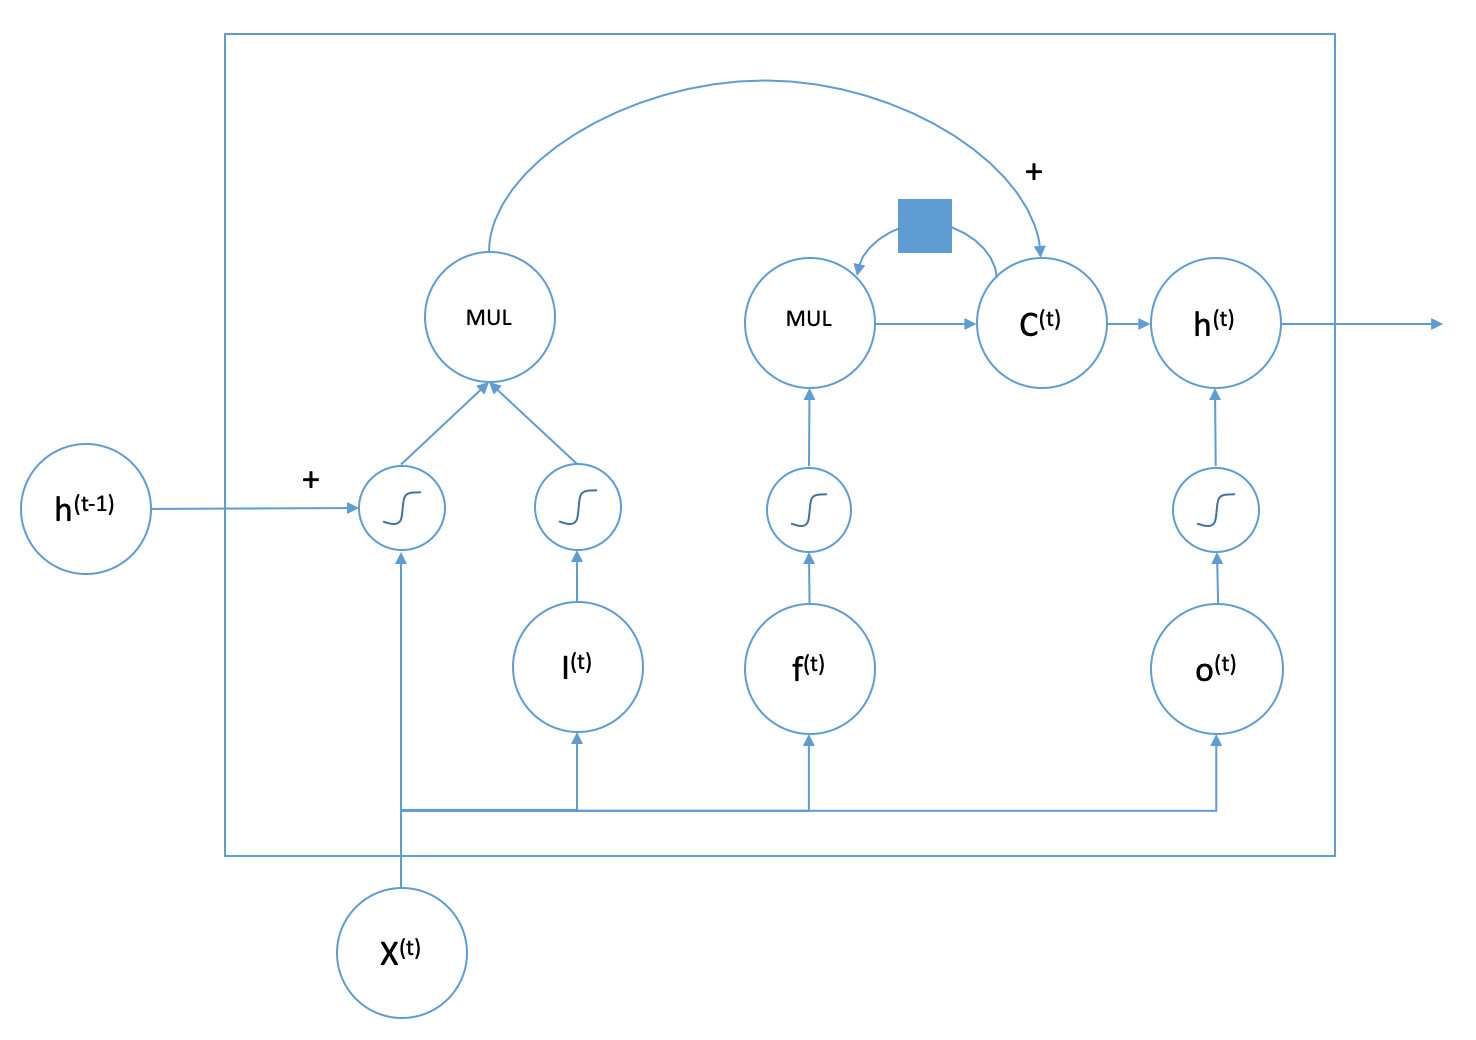
\includegraphics[width=\textwidth]{capitulo2/images/lstm}
   		\caption{Una compuerta LSTM típica.}
   		\label{fig:lstm}
   	\end{figure}
   	
   	

\newpage
\subsection{Aprendizaje profundo como servicio}
El entrenamiento de redes neuronales profundas, conocidas como aprendizaje profundo es en la actualidad áltamente complejo computacionalmente. Requiere un sistema con la combinación correcta de software, drivers, memoria, red y recursos de almacenamiento, por factores como estos los proveedores de cloud computing como Amazon Web Services, Microsoft Azure o Google Cloud ofrecen actualmente servicios de Machine Learning proveyendo API's como pueden ser de entrenamiento de modelos o de visualización de datos y generación de estadísticas, permitiendo que desarrolladores y científicos de datos se enfoquen mas en tareas como el entrenamiento de modelos, análisis de datos, etc.
\\\\
Los modelos de aprendizaje profundo requieren de un proceso experimental e iterativo, requiriendo cientos e incluso miles de ejecuciones que requieren de un amplio poder de cómputo para encontrar la combinación correcta de las configuraciones e hiper-parámetros de la red neuronal. Esto puede tomar semanas o incluso meses y este tipo de servicios garantiza una disponibilidad en todo momento y en conjunto permite que un sistema completo esté dividido en módulos consiguiendo que el mantenimiento y detección de fallos sean tareas más sencillas.
\\\\ 
En la figura \ref{fig:DLAAS} se puede observar la arquitectura de un sistema divido en módulos y que hace uso de herramientas de Machine Learning para dar respuesta a otros módulos del sistema.

\begin{figure}[H]
	\centering
	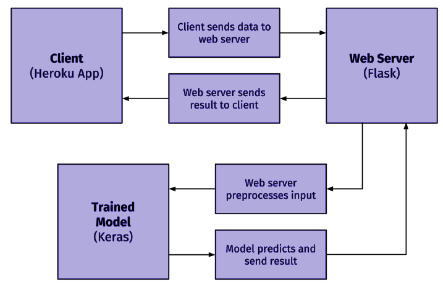
\includegraphics[width=0.7\textwidth]{capitulo2/images/DLAAS.png}
	\caption{Ejemplo de sistema con módulo de Machine Learning}
	\label{fig:DLAAS}
\end{figure}

%==============================================================

\section{Métodos de reconocimiento de expresiones matemáticas}
\subsection{Análisis sintáctico dirigido}
Los lenguajes libres de contexto, son aquellos que tienen una notación recursiva natural llamada \textit{gramática libre de contexto}. Por ende, un lenguaje libre de contexto es todo aquel que puede ser representado por una gramática libre de contexto.

Una gramática libre de contexto G, queda definida de la siguiente manera:

\begin{equation}
G = (V, T, P, S)
\end{equation}

de donde, V es el conjunto de variables, T el conjunto de símbolos terminales, P el conjunto de producciones y S el punto de inicio \cite{automata}.

El lenguaje matemático, es decir, las expresiones matemáticas son un lenguaje libre de contexto. Esto quiere decir que es posible definir una gramática libre de contexto para definir a las expresiones matemáticas. Esta es una práctica muy común en la teoría de compiladores.

Sabiendo esto, una aproximación a la resolución del problema de reconocer expresiones matemáticas en imágenes es la que describe \cite{gramaticasAnderson}. El método consiste en dos etapas:

\begin{itemize}
	\item Reconocimiento de caracteres: Utilizar algún método de reconocimiento de patrones para localizar los caracteres y anotar sus coordenadas. 
	\item Análisis sintáctico dirigido: Utilizar la etapa previa para determinar la jerarquía, basándose en un conjunto de reglas definidas (las gramáticas libres de contexto).
\end{itemize}

En la Figura \ref{fig:gramaticas}, se puede ver un ejemplo del proceso de reconocimiento propuesto por este método.

\begin{figure}[h]
	\centering
	\subfigure[]{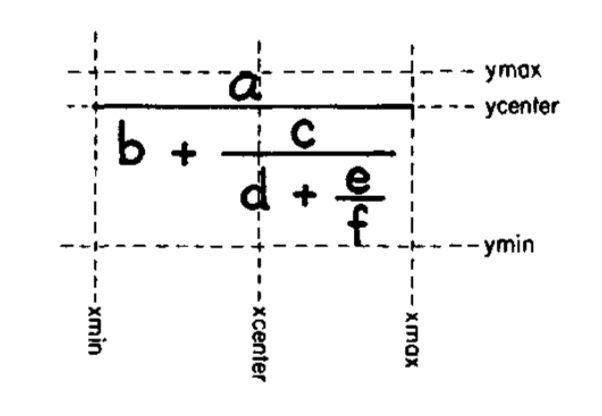
\includegraphics[width=6cm]{capitulo2/images/gramaticas1}}
	\subfigure[]{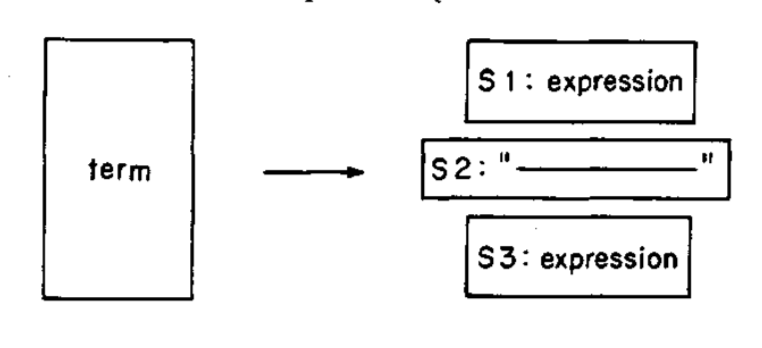
\includegraphics[width=6cm]{capitulo2/images/gramaticas2}}
	\caption{\textbf{a)} La primera etapa del método de reconocimiento, se anotan las coordenadas de de cada caracter. \textbf{b)} Se realiza un análisis sintáctico con las gramáticas libres de contexto definidas.}
	\label{fig:gramaticas}
\end{figure}

\subsection{Análisis estructural}

Este método coincide con el primero en que debe de utilizar una técnica de reconocimiento de patrones para etiquetar primero los símbolos. Las etiquetas que utiliza tienen que ver son su posición en la imagen, así como su tamaño. 

La diferencia en este método, radica en su segunda etapa. No se realizará un análisis con gramáticas, en su lugar se intentara deducir la estructura jerárquica con algún otro método. El artículo \cite{spanningtree} propone utilizar el algoritmo de Kruskal para obtener un árbol de recubrimiento mínimo por niveles, de este modo se puede saber la estructura de la expresión matemática recorriendo el gráfo resultante.La Figura \ref{fig:spanningtree} muestra un ejemplo de como funciona este método.

\begin{figure}[h]
	\centering
	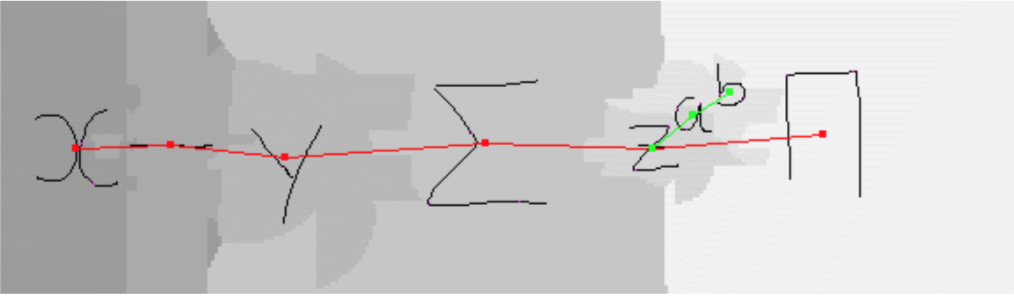
\includegraphics[width=8cm]{capitulo2/images/spanningtree}
	\caption{Utilización de un árbol de recubrimiento mínimo para el reconocimiento de expresiones matemáticas.}
	\label{fig:spanningtree}
\end{figure}


\subsection{Image Captioning}

Es una rama emergente del \textit{deep learning} que ha ido ganando atención en los últimos años. Este campo es un punto intermedio entre la vision por computadora y el procesamiento del lenguaje natural. El actual estado del arte en image captioning tiene una aproximación similar a los modelos sequence-to-sequence, los cuales utilizan una arquitecura Encoder-Decoder \cite{imagetolatex}.

Si se trata al problema de reconocer expresiones matemáticas en imagenes como un problema sequence-to-sequence de image captioning, se puede emplear una arquitectura de Encoding-Decoding para hacer la conversión de la imagen a LaTeX de manera directa. Esto permite a la red manejar imagenes de longitud variable y reconocer los símbolos a la vez que va reconociendo las expresiones.

La arquitectura que se esta utilizando actualmente para solucionar este problema se muestra en la Figura \ref{fig:imgcaptioning} \cite{imagetolatex}\cite{imagemarkup}\cite{chino}.

\begin{figure}
	\centering
	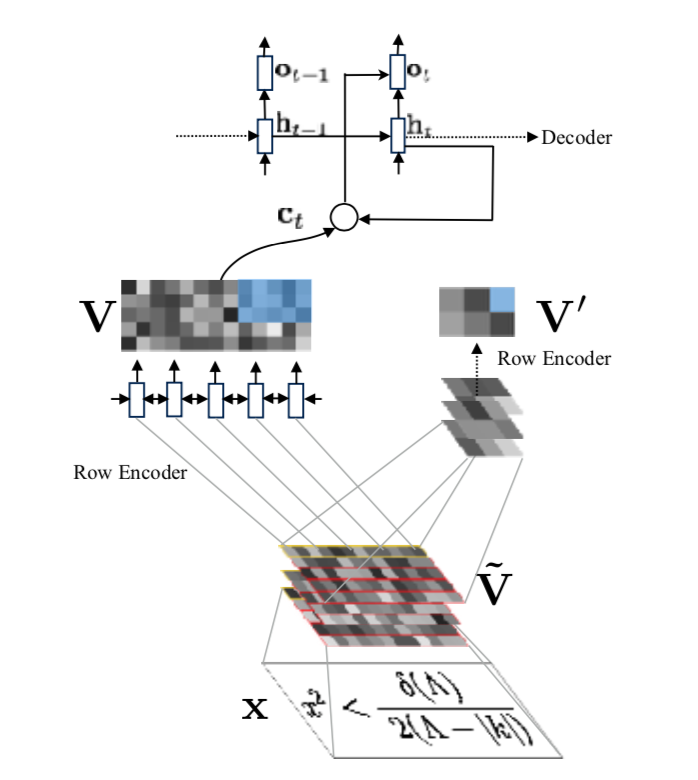
\includegraphics[width=8cm]{capitulo2/images/imgcaptioning}
	\caption{Arquitectura de image captioning para reconocer expresiones matemáticas en imagenes.}
	\label{fig:imgcaptioning}
\end{figure}

%==============================================================

\section{Aplicación web}
En la ingeniería de software se denomina aplicación web a aquellas herramientas que los usuarios pueden utilizar accediendo a un servidor web a través de internet o de una intranet mediante un navegador. En otras palabras, es un programa que se codifica en un lenguaje interpretable por los navegadores web en la que se confía la ejecución al navegador \cite{appweb}.

\subsection{Django}
Django es un framework de desarrollo web completamente desarrollado en Python. Permite de una manera rápida poder implementar una aplicación web en el lenguaje Python. Las siguientes, son de las principales características de Django:

\begin{itemize}
    \item \textbf{Rápido}: Tiene como filosofía ayudar a los desarrolladores a crear aplicaciones en el menor tiempo posible.
    \item \textbf{Completo}: Incluye cientos de librerías que permiten ahorrar tiempo y automatizar tareas.
    \item \textbf{Seguro}: Es una de las principales características de Django ya que incluye soluciones a los principales ataques que puede sufrir una aplicación web.
    \item \textbf{Escalable}: Con el patrón de diseño de Django es posible incrementar o decrementar la capacidad de un sitio.
    \item \textbf{Versátil}: Es utilizado por muchas empresas y organizaciones a lo largo del mundo para crear diferentes tipos de proyectos.
\end{itemize}

\subsubsection{Modelo-Vista-Template}
El Modelo-Vista-Template (MTV) es el patrón de diseño que Django implementa. Este patrón es una modificación al conocido Modelo-Vista-Controlador (MVC). La diferencia radica en que Django se encarga de hacer la parte del controlador, por ende el desarrollador solamente tiene que preocuparse por implementar la lógica de negocio y de como mostrará los datos. En la Figura \ref{fig:mtv}, se puede ver una representación del patrón MTV. En el patrón de diseño MTV \cite{mtv}:

\begin{figure}
    \centering
    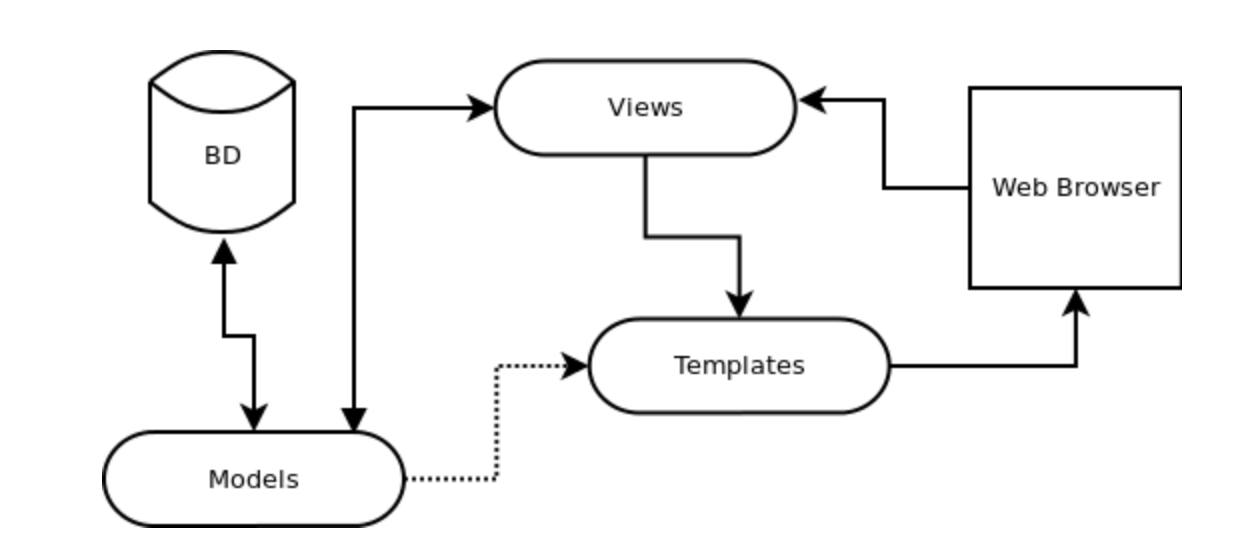
\includegraphics[width=\textwidth]{capitulo2/images/mtv.png}
    \caption{Representación del patrón de diseño Modelo-Vista-Template.}
    \label{fig:mtv}
\end{figure}

\begin{itemize}
    \item \textbf{Modelo}: La capa de acceso a la base de datos. Esta capa contiene toda la información sobre los datos: cómo acceder a estos, cómo validarlos, cuál es el comportamiento que tiene, y las relaciones entre los datos.
    \item \textbf{Template}: La capa de presentación. Esta capa contiene las decisiones relacionadas a la presentación: como algunas cosas son mostradas sobre una página web o otro tipo de documento.
    \item \textbf{Vista}: La capa de la lógica de negocios. Esta capa contiene la lógica que accede al modelo y la delega a la plantilla apropiada: puedes pensar en esto como un puente entre el modelos y las plantillas.
\end{itemize}

\subsection{API REST}
\subsubsection{Application Programming Interface}
Una Interfaz de Programación de Aplicaciones o API es un conjunto de definiciones y protocolos que se utilizan para desarrollar e integrar el software de las aplicaciones.

Las API permiten que sus servicios se comuniquen con otros, sin necesidad de saber como están implementados. Esto simplifica el desarrollo de las aplicaciones y permite ahorrar tiempo y dinero \cite{apiArticle}.
\subsubsection{Represenational State Transfer}

Representational State Transfer (REST) es un estilo de arquitectura basado en un conjunto de principios que describen como recursos interconectados son definidos y direccionados. Estos principios fueron descritos en el año 2000 por Roy Fielding como parte de obtención de su doctorado.
\\
Es importante hacer énfasis en que REST es un \textbf{estilo de software de arquitectura} y no un conjunto de estandares. Como resultado, dichas aplicaciones o arquitecturas son en ocasiones referidas como aplicaciones RESTful o REST-style \cite{restArticle}. 
\\
Una aplicación o arquitectura considerada RESTful o REST-style es caracterizada por:
\begin{itemize}
	\item La funcionalidad y estado son dividiad en recursos distribuidos.
	\item Cada recurso es únicamente direccionable usando un conjunto uniforme y mínimo de comandos (típicamente usando comandos HTTP de GET, POST, PUT o DELETE).
	\item El protocolo es cliente/servidor, stateless, por capas y soporta almacenamiento cache.
\end{itemize} 
 La figura \ref{fig:rest_mess} ilustra el uso de REST para servicios Web.
\begin{figure}[H]
	\centering
	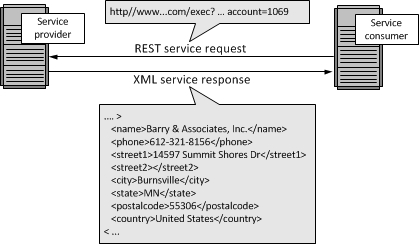
\includegraphics[width=0.5\textwidth]{capitulo2/images/rest_messages.jpg}
	\caption{Consumidor y proveedor de servicios comunicandose mediante solicitudes y respuestas REST.}
	\label{fig:rest_mess}
\end{figure}  
\subsubsection{Autentificación}
Para hablar de autentificación es necesario primero entender la diferencia entre identificación y autentificación, por un lado la identificación es la capacidad de identificar de forma exclusiva a un usuario de un sistema o una aplicación que se está ejecutando, mientras que la autentificación es la capacidad de demostrar que un usuario o una aplicación es quien dicha persona o aplicación asegura ser \cite{authent}.\\\\
Para el caso de una REST API es en muchas ocasiones necesario que se lleve a cabo la autentificación para permitir o denegar el acceso a recursos de un servidor por ejemplo de acuerdo a los permisos concedidos en función de las credenciales de autentificación para así asegurar que los datos sean visibles únicamente a aquellos que proporcionen las credenciales adecuadas y dispongan de los permisos necesarios.

%https://www.ibm.com/support/knowledgecenter/es/SSFKSJ_7.5.0/com.ibm.mq.sec.doc/q009740_.htm
\section{Android}
Esta sección tiene objetivo presentar las principales características en el desarrollo de la aplicación para Android.
\subsection{Arquitectura de la aplicación}
Para el desarrollo de la aplicación se implemento la arquitectura Clean, la cual como ya se ha mencionado antes se ha mencionado se ha vuelto muy popular en el desarrollo de aplicaciones móviles para android debido a que es una solución que produce sistemas que presentan las siguientes características.

\begin{itemize}
    \item Escalables, por lo que se pueden agregar más funcionalidades de forma sencilla.
    \item Presentan modularidad.
    \item Presentan independencia en cuanto a frameworks, interfaz de usuario y bases de datos.
    \item El proyecto es más fácil de mantener por lo que es más sencillo hacer cambios.
\end{itemize}

Al utilizar esta arquitectura el proyecto queda separado en tres capas como se observa en la figura \ref{fig:capas-arquitectura} con lo cual cada una de ellas tiene su propósito definido.

\begin{figure}[h]
    \centering
    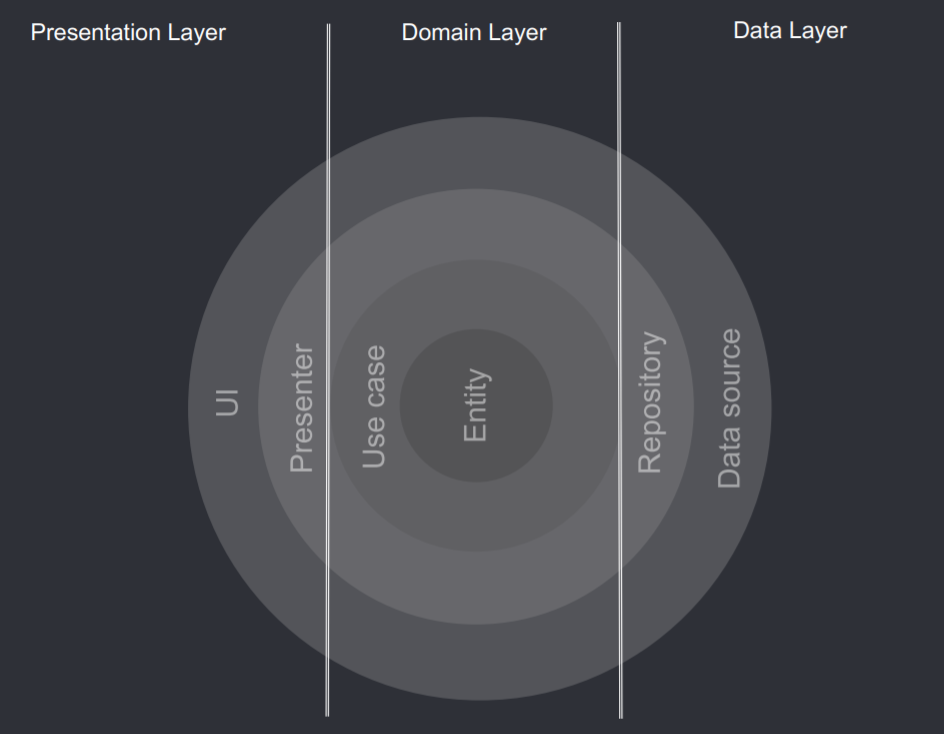
\includegraphics[width=250px]{capitulo5/android/img/capas-clean.png}
    \caption{Tres capas que se tienen al utilizar la arquitectura Clean \cite{cleanGuide}}
    \label{fig:capas-arquitectura}
\end{figure}

\subsubsection{Capa de datos}
La información que se utiliza en el resto de capas proviene de esta capa. Esta capa a su vez se encuentra dividida en la capa de repositorio y en la capa de fuente de datos. 

\paragraph{Capa de repositorio} En esta capa se utiliza el patrón de repositorio como se muestra en la figura \ref{fig:capa-datos}. Gracias a este patrón se puede tener acceso a diferentes fuentes de datos que se encuentran en la capa más baja de nuestra arquitectura, esto nos permite un acceso a los datos de forma transparente para el usuario bajo las condiciones que se presenten.

La forma de utilizar este patrón en la aplicación desarrollado crear una clase en la cual se hace uso de la interfaz que se tiene para el acceso a la fuente de datos. En el siguiente código se puede apreciar el como se crea una instancia de APIService que es nuestra interfaz para fuente de datos.

Después, en nuestro método findAllProyecttosByUser se recupera la información necesaria para mandarla a las capas superiores.

\lstinputlisting[language=Java]{capitulo5/android/src/repositorio.java}

\begin{figure}[h]
    \centering
    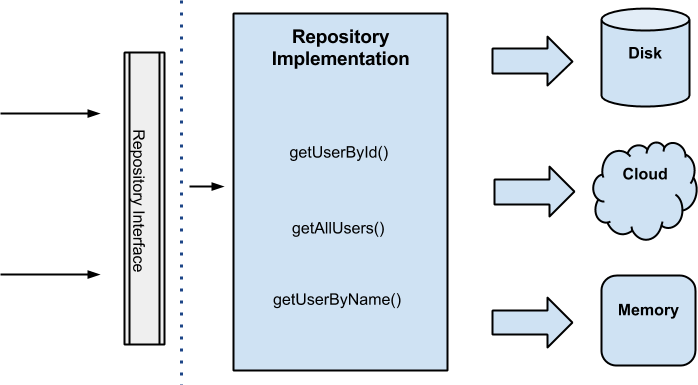
\includegraphics[width=400px]{capitulo5/android/img/capa-datos.png}
    \caption{Capa de datos \cite{cleanWay}}
    \label{fig:capa-datos}
\end{figure}

\paragraph{Capa de fuente de datos} En este trabajo, la fuente de datos que se tiene es un API REST, sin embargo si se requiere acceder a información que se persista en el teléfono se pude agregar otra fuente de datos. Se utilizó retrofit para poder realizar la comunicación con el API REST. 

La forma de utilizar retrofit es crear una interfaz con todos los métodos para recuperar o enviar información al API REST, en esta interfaz cada método tiene la URL a la cual se realizara la petición con alguno de los métodos que tiene HTTP, se tienen los parámetro que se envían y cada método nos regresa una llamada asíncrona que se trabaja en la capa de repositorio. Esto se puede apreciar en el siguiente código.

\lstinputlisting[language=Java]{capitulo5/android/src/APIService.java}

Para poder hacer uso de esta interfaz se tiene que configurar bajo ciertas características especificas como lo son la URL a la cual hará peticiones, el logger que se utilizara para poder observar las peticiones que se realizan y brindar una retroalimentación a la hora de hacer pruebas y por ultimo el parser que se utilizara para trabajar y pasar de clases a datos que el API REST entienda y pueda utilizar, en este caso se utilizo el formato JSON. La definición de estas características se tiene en el siguiente código.

\lstinputlisting[language=Java]{capitulo5/android/src/ServiceGenerator.java}

Finalmente, en esta capa se tienen clases Java que después se mapean a objetos JSON y viceversa, para realizar esto se crea un POJO con los atributos que se necesitan además de agregar anotaciones de retrofit para que el parser pude hacer la conversión necesaria. Un ejemplo de esto es en la siguiente clase de java.

\lstinputlisting[language=Java]{capitulo5/android/src/UsuarioData.java}


\subsubsection{Capa de dominio}
En esta capa es la intermediaria entre las otras dos capas que se tienen, es donde se encuentran los casos de uso también conocidos como interactors como se muestra en la figura \ref{fig:capa-dominio} en ellos la lógica del negocio es ejecutada es por esto que es el núcleo de la aplicación.

Es importante mencionar que esta capa, al ser la encargada del negocio es donde se hacen validaciones en la información y dicha información se adapta para que sea trabajada en la capa de presentación o en la de datos

Además de contener los casos de uso en esta capa se encuentran las entidades y se hace uso de los repositorios para acceder a la información proporcionada por la capa de datos.

\begin{figure}[h]
    \centering
    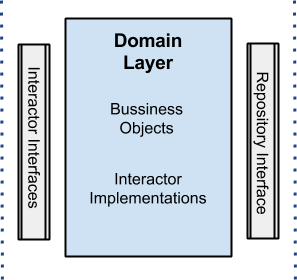
\includegraphics[width=200px]{capitulo5/android/img/capa-dominio.png}
    \caption{Capa de dominio \cite{cleanWay}}
    \label{fig:capa-dominio}
\end{figure}

Para tener un control sobre posibles errores en la capa de presentación o en la capa de datos se utilizan códigos de resultados al igual que una clase que contiene el resultado que se puede presentar, así como la información que se le regresa a la capa de presentación. Se hace uso de genéricos para poder reutilizar esta clase en toda la aplicación y no duplicar código. La clase es la siguiente.

\lstinputlisting[language=Java]{capitulo5/android/src/BusinessResult.java}

La forma en la que se utiliza esta clase en un caso de uso se presenta en el siguiente código que permite iniciar sesión.

\lstinputlisting[language=Java]{capitulo5/android/src/UserInteractorImpl.java}

A su vez el caso de uso utiliza sus propios clases de java para presentar información al usuario en la capa de presentación así como controlar posibles errores en la información que ingrese el usuario los campos de los formularios, un ejemplo de este tipo de clases es el siguiente.

\lstinputlisting[language=Java]{capitulo5/android/src/UsuarioModel.java}

\subsubsection{Capa de presentación}
En esta capa como se muestra en la figura \ref{fig:capa-presentacion} se trabaja con la lógica relacionada a las interfaces que se tienen en la aplicación, es decir a actividades, fragmentos y archivos XML.

\begin{figure}[h]
    \centering
    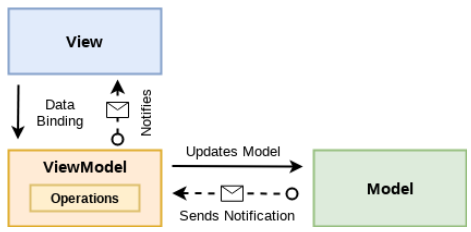
\includegraphics[width=300px]{capitulo5/android/img/capa-presentacion.png}
    \caption{Capa de presentación \cite{cleanWayReload}}
    \label{fig:capa-presentacion}
\end{figure}

En esta capa se pueden trabajar con patrones como MVC y MVP pero en este caso se utiliza el patrón MVVM cada uno con una función en particular. \cite{cleanWayReload}

\begin{itemize}
    \item \textbf{Modelo} Se encarga de representar la información que sera presentada en la vista.
    \item \textbf{Vista} Compuesta en este caso por las actividades y fragmentos de la aplicación, su tarea es mostrar la información, hacen uso de los viewmodels para poder realizar cambios en la interfaz.
    \item \textbf{ViewModel} El ViewModel sera el encargado de ejecutar los casos de uso o interactors con el objetivo de actualizar la vista de acuerdo a la información que presente el modelo.
\end{itemize}


